% generated by scripts/pkl_to_latex.py
% source PKL : thermal_v1_L6_Ne4_U10_t1_mode-uniform_tpall_t2all_tperpall_nmin2_solver-gcg_full_restarts10_iter300_kmax4_tol1em09_cut10_adaptive1_step5_clusteravg1_T0to1_N40-98c4f0fd07f2_knone_diag0.pkl
% scan type  : Tscan
% state      : gs
% requires   : \usepackage{pgfplots} \pgfplotsset{compat=1.18}
% colours match the matplotlib PDF (tab10 cycle)
\definecolor{gmeC0}{HTML}{1F77B4}
\definecolor{gmeC1}{HTML}{FF7F0E}
\definecolor{gmeC2}{HTML}{2CA02C}
\definecolor{gmeC3}{HTML}{D62728}
\definecolor{gmeC4}{HTML}{9467BD}
\definecolor{gmeC5}{HTML}{8C564B}
\definecolor{gmeC6}{HTML}{E377C2}
\definecolor{gmeC7}{HTML}{17BECF}

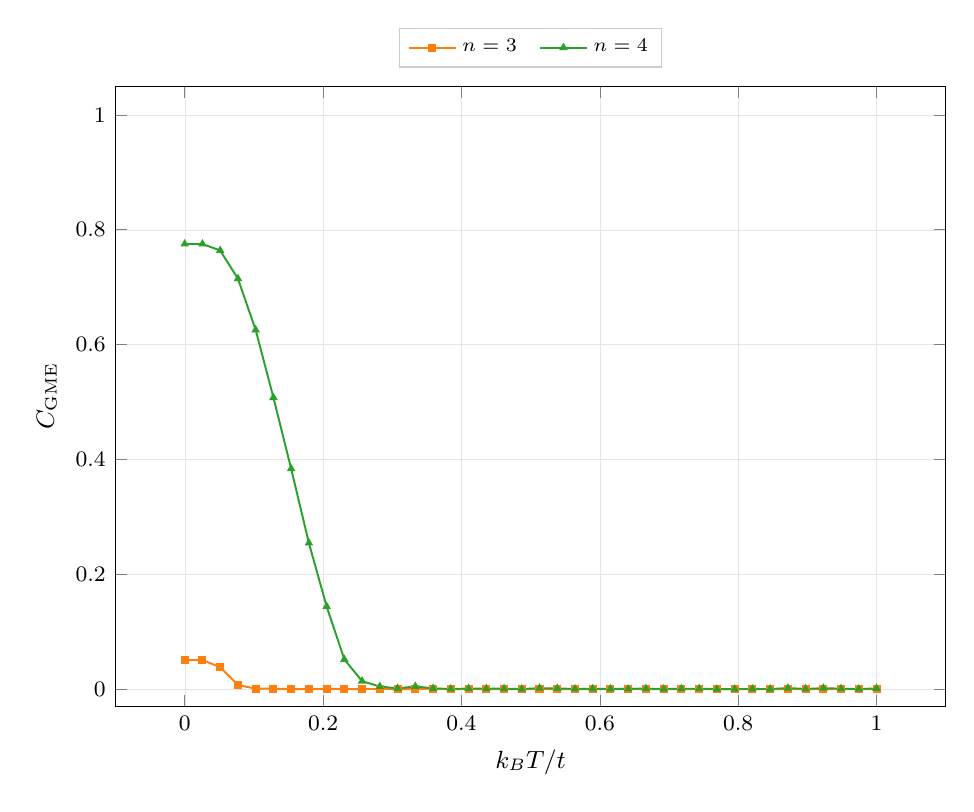
\begin{tikzpicture}
  \begin{axis}[
    width=\columnwidth,
    height=0.78\columnwidth,
    xlabel={$k_B T/t$},
    ylabel={$C_{\mathrm{GME}}$},
    grid=both,
    grid style={line width=.1pt, draw=gray!20},
    tick label style={font=\footnotesize\rmfamily, /pgf/number format/fixed},
    label style={font=\small\rmfamily},
    scaled ticks=false,
    legend style={font=\scriptsize\rmfamily, draw=gray!40, at={(0.5,1.03)}, anchor=south, /tikz/every even column/.append style={column sep=6pt}},
    legend cell align={left},
    legend columns=2,
    ymin=-0.03,
    ymax=1.05,
  ]
    \addplot[color=gmeC1, mark=square*, mark size=1.1pt, line width=0.7pt] coordinates {
        (0,0.050632) (0.025641,0.050589) (0.051282,0.038179) (0.076923,0.00718)
        (0.102564,0.000735) (0.128205,0.000672) (0.153846,0.000087) (0.179487,0.000017)
        (0.205128,0.000348) (0.230769,0.000177) (0.25641,0.000043) (0.282051,0.000245)
        (0.307692,0.000014) (0.333333,0.000021) (0.358974,0.000875) (0.384615,0.000012)
        (0.410256,0.000224) (0.435897,0.000016) (0.461538,0.000069) (0.487179,0)
        (0.512821,0.000005) (0.538462,0.000037) (0.564103,0.000049) (0.589744,0.000018)
        (0.615385,0.000044) (0.641026,0.00038) (0.666667,0) (0.692308,0.000095)
        (0.717949,0.000008) (0.74359,0.000144) (0.769231,0.000035) (0.794872,0.000004)
        (0.820513,0) (0.846154,0.000001) (0.871795,0.000035) (0.897436,0.000098)
        (0.923077,0.00001) (0.948718,0.000001) (0.974359,0.000005) (1,0.000056)
    };
    \addlegendentry{$n=3$}
    \addplot[color=gmeC2, mark=triangle*, mark size=1.1pt, line width=0.7pt] coordinates {
        (0,0.775145) (0.025641,0.775142) (0.051282,0.763812) (0.076923,0.714771)
        (0.102564,0.625559) (0.128205,0.50776) (0.153846,0.383859) (0.179487,0.254492)
        (0.205128,0.144009) (0.230769,0.05168) (0.25641,0.013822) (0.282051,0.004537)
        (0.307692,0.001155) (0.333333,0.004718) (0.358974,0.001147) (0.384615,0.000186)
        (0.410256,0.000945) (0.435897,0.000721) (0.461538,0.000771) (0.487179,0.000077)
        (0.512821,0.00166) (0.538462,0.001102) (0.564103,0.000283) (0.589744,0.000541)
        (0.615385,0.0003) (0.641026,0.000359) (0.666667,0.000934) (0.692308,0.000047)
        (0.717949,0.000648) (0.74359,0.000642) (0.769231,0.000015) (0.794872,0.000032)
        (0.820513,0.000361) (0.846154,0.000101) (0.871795,0.00179) (0.897436,0.00024)
        (0.923077,0.001621) (0.948718,0.000782) (0.974359,0.000165) (1,0.00116)
    };
    \addlegendentry{$n=4$}
  \end{axis}
\end{tikzpicture}
